\documentclass[10pt,twocolumn,a4paper]{article}
\usepackage[T1]{fontenc}
\usepackage{times}
\usepackage[margin=2cm,columnsep=0.7cm]{geometry}
\usepackage{microtype}
\usepackage{graphicx}
\usepackage{booktabs}
\usepackage{amsmath}
\usepackage[numbers,sort&compress]{natbib}
\usepackage[font=small,labelfont=bf,skip=4pt]{caption}
\usepackage{enumitem}
\usepackage{titlesec}
\usepackage{xcolor}
\usepackage[colorlinks=true,linkcolor=black,citecolor=black,urlcolor=blue!50!black]{hyperref}
\setlist{nosep,leftmargin=*}
\titleformat{\section}{\normalfont\large\bfseries}{\thesection}{0.6em}{}
\titleformat{\subsection}{\normalfont\normalsize\bfseries}{\thesubsection}{0.6em}{}
\titlespacing*{\section}{0pt}{8pt}{3pt}
\titlespacing*{\subsection}{0pt}{6pt}{2pt}
\newcommand{\LUE}{LUE$_x$}

\title{\vspace{-1.2em}\textbf{Does Seeing the Search Result Make Tool Utility Predictable?}\\[2pt]
\large A diagnostic follow-up to \textit{To Call or Not to Call}}
\author{Anchal Singh Parihar\\ \small SRM University, Sonipat, India}
\date{\small October 2026}

\begin{document}
\maketitle

\begin{abstract}
\citet{wu2026tocall} find that probes on an LLM's hidden state predict whether a tool is \emph{needed} well, but whether calling it will \emph{help} much less well. We ask whether this gap comes from noisy utility labels, and how much it closes once the probe can see the retrieved results. On Llama-3.2-3B-Instruct with forced Google search on BFCL, utility labels are highly consistent across judge repeats (Fleiss $\kappa = 0.97$). A probe on the post-search state predicts utility better than one on the pre-search state (AUROC $0.60 \rightarrow 0.75$; $+0.15 \pm 0.03$ over 10 seeds) and beats text-only baselines on the same prompt. However, the gain is explained by need and answer correctness: the product of a pre-search need probe and a post-search correctness probe predicts utility at least as well (0.80 vs.\ 0.75). The post-search state mainly encodes whether the upcoming answer will be correct, which is close to whether the answer string appears in the snippets. Every number in this report is regenerated from the raw run files by released scripts.
\end{abstract}

\section{Introduction}
Tool-augmented LLMs must decide when a tool call is worth its cost. \citet{wu2026tocall} separate this decision into \emph{need} (the model would fail without the tool) and \emph{utility} (the tool call would turn a wrong answer into a right one), and train MLP probes on hidden states to predict both. On web-search tasks, need probes (LNE) are accurate, while utility probes (\LUE) are weaker; for Llama-3.2-3B on BFCL the paper reports AUROC $0.812 \pm 0.039$ and $0.723 \pm 0.024$. The paper attributes the gap to utility depending on the tool output, which the model has not seen when it decides.

We test this explanation directly with two questions.
\textbf{Q1.} Are the utility labels themselves noisy enough to cap probe performance?
\textbf{Q2.} If the probe reads the hidden state \emph{after} the search results are in the prompt, how much does utility prediction improve, and what signal is responsible?

Our contributions are: (i) a replication of the paper's need and utility probes with its released harness; (ii) a label-reliability analysis; (iii) a pre- vs.\ post-search comparison with controls for seed, label permutation, text-only shortcuts and the need $\times$ correctness structure of the label; and (iv) the identification of a silent tool-argument failure affecting 19\% of forced-search runs in the base harness loop.

\section{Setup}
\textbf{Model, task and harness.} We use Llama-3.2-3B-Instruct on the 314 BFCL web-search questions (308 distinct question strings) with the authors' harness \citep{wu2026tocall}: one run without tools and one with forced Google search (SerpAPI, October 2026), temperature 0. We use the base local loop rather than the chat-template harness the paper uses for this model; a 50-question pilot with the chat template returned raw tool-call JSON as the final answer (accuracy 0.24).

\textbf{Labels.} Answers are scored with the paper's BFCL judge prompt on Qwen2.5-7B-Instruct (4-bit, $K = 3$ repeats) instead of GPT-4o. \emph{Need} $= 1$ if the no-tool answer is wrong; \emph{utility} $= 1$ if the search answer is right and the no-tool answer is wrong. With binary scores, utility $=$ need $\times$ correct, where \emph{correct} refers to the search answer.

\textbf{Probes.} Following the paper's App.~E, we train MLP probes (hidden sizes $\{(),128,256,(128,64),(1024,64)\}$, learning rates $\{10^{-3},10^{-4}\}$) on the standardised last-token, final-layer state, with nested 5-fold stratified cross-validation and identical outer folds for all probes. \emph{PRE} is the state at the end of the no-tool prompt (the paper's \LUE{} input); \emph{POST} is the state at the end of the forced-search final prompt, which contains the snippets. We report pooled out-of-fold AUROC with question-level bootstrap CIs and paired bootstrap tests, and, for comparison with the paper, the mean $\pm$ SD of per-fold AUROC.

\textbf{Clean set.} Of the 314 runs, 60 passed the wrong argument name to the search tool and received an error string instead of results (Sec.~\ref{sec:data}), and 22 questions refer to an unnamed entity (``Where is his hometown?''). Because an error string is a trivial cue that search did not help, our main results use the 229 remaining questions with hidden states; we report the full set ($n = 308$) alongside. The rule was fixed after inspecting accuracy by failure type, so it is post hoc.

\section{Results}
\subsection{Q1: label reliability}
Across three judge repeats, utility labels have Fleiss $\kappa = 0.97$ [0.94, 0.99] and a per-question flip rate of 0.02 on the clean set (full set: $\kappa = 0.96$). Repeat-to-repeat noise therefore cannot explain a utility AUROC of 0.60--0.72. Consistency is not correctness: a second LLM (Claude), blind to the judge, labelled a stratified sample of 50 answers and agreed on 45 (0.90, Cohen's $\kappa = 0.80$); the judge erred on the strict side in most disagreements. No human labels were collected.

\subsection{Q2: pre- vs.\ post-search state}
\begin{figure}[t]
\centering
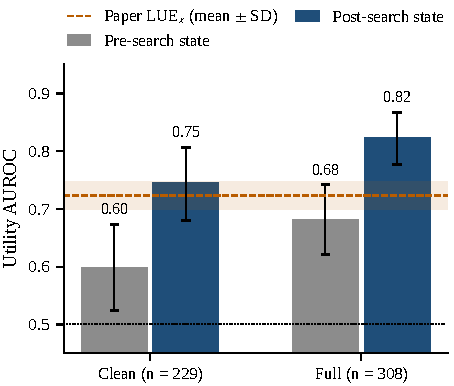
\includegraphics[width=\columnwidth]{../figures/fig1_auroc.pdf}
\caption{Utility AUROC of probes on the pre- and post-search hidden state (seed 42, 95\% bootstrap CIs). The shaded band is the paper's \LUE{} for the same model and task.}
\label{fig:auroc}
\end{figure}

Figure~\ref{fig:auroc} shows the main comparison. On the clean set, utility AUROC rises from 0.60 [0.52, 0.67] (PRE) to 0.75 [0.68, 0.81] (POST), a paired difference of $+0.15$ [0.06, 0.24]. On the full set it rises from 0.68 to 0.82 ($+0.14$ [0.07, 0.21]); this POST number is inflated by the error strings in 60 prompts. The need probe reaches 0.90 (full: 0.91).

\textbf{Relation to the paper.} With the paper's aggregation, our full-set PRE utility probe gives $0.69 \pm 0.07$, within about one SD of the paper's $0.72 \pm 0.02$. On the clean set it is lower and unstable across folds ($0.63 \pm 0.15$; per-fold range 0.42--0.79). Our need probe is higher than the paper's ($0.93 \pm 0.03$ vs.\ $0.81 \pm 0.04$), and our judge also marks more no-tool answers wrong (need rate 0.88, against about 0.83 implied by the paper's no-tool accuracy of 0.17). The judge, harness and search date all differ, so we compare the size of the effect, not exact values.

\begin{figure}[t]
\centering
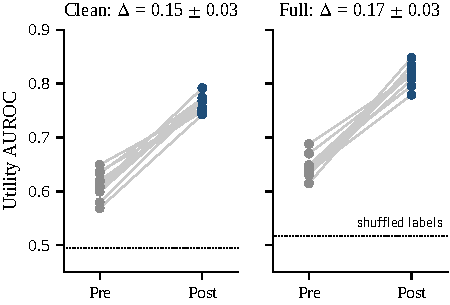
\includegraphics[width=\columnwidth]{../figures/fig2_seeds.pdf}
\caption{PRE and POST utility AUROC for 10 probe seeds (lines pair the same seed). Dotted line: mean POST AUROC with shuffled labels (20 permutations).}
\label{fig:seeds}
\end{figure}

\textbf{Robustness.} Over 10 seeds (Fig.~\ref{fig:seeds}) the gain is $+0.15 \pm 0.03$ on the clean set (minimum $+0.11$) and $+0.17 \pm 0.03$ on the full set (minimum $+0.13$); it is positive for every seed. With shuffled labels, the POST probe scores 0.49 (clean) and 0.52 (full), so the pipeline does not leak labels.

\subsection{What signal explains the gain?}
\begin{figure*}[t]
\centering
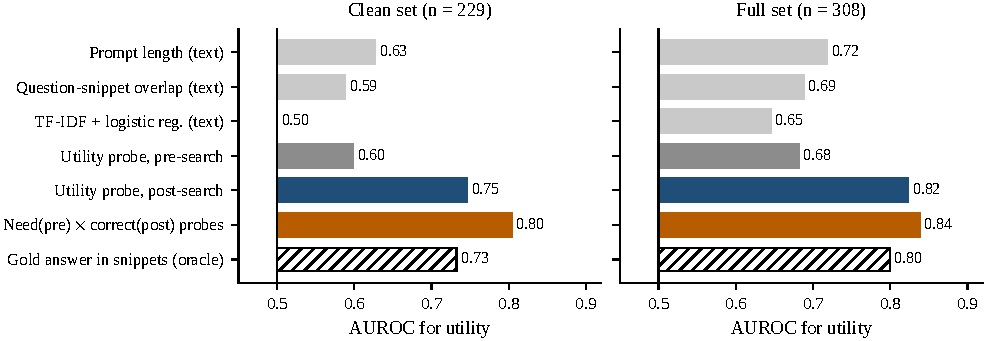
\includegraphics[width=0.92\textwidth]{../figures/fig3_decomposition.pdf}
\caption{Predictors of utility on the same questions. Grey: text-only baselines on the post-search prompt (TF-IDF uses the same outer folds as the probes). Orange: product of the out-of-fold need probability from PRE and the out-of-fold correctness probability from POST. Hatched: whether all gold-answer tokens appear in the prompt; it uses the gold answer and is a reference, not a baseline.}
\label{fig:decomp}
\end{figure*}

A higher POST AUROC could come from prompt format rather than content, or from the probe recognising that the next answer will be correct. Figure~\ref{fig:decomp} separates these.

\textbf{Text-only shortcuts.} On the clean set, prompt length (0.63), question--snippet overlap (0.59) and a TF-IDF logistic regression (0.50 [0.42, 0.58]) are all below the POST probe (0.75). The probe is not reproducing a surface feature of the prompt.

\textbf{Inside need $= 1$.} Where the no-tool answer is wrong ($n = 202$), utility equals correctness, so need cannot contribute. The gain persists: $0.65 \rightarrow 0.84$, $+0.19$ [0.11, 0.28] (full: $+0.20$ [0.13, 0.26]).

\textbf{Need $\times$ correctness.} The POST state predicts whether the search answer is correct with AUROC 0.82 (full: 0.87), while PRE predicts need with 0.90. Multiplying the two out-of-fold probabilities predicts utility with AUROC 0.80, which is \emph{higher} than the POST utility probe by 0.06 [0.01, 0.11] on the clean set; on the full set the two are indistinguishable (0.84 vs.\ 0.82, difference $-0.01$ [$-0.06$, 0.03]). The POST utility probe therefore carries no detectable signal beyond need and answer correctness. Correctness itself is close to a lexical property of the evidence: whether the gold answer appears in the snippets reaches 0.73 for utility on the clean set.

\textbf{Interpretation.} Utility is hard to predict before the search because it depends on whether the search will return the answer. Once the answer is in the context, the hidden state reflects whether the model is about to answer correctly, in line with prior work showing that LLMs encode their own answer correctness \citep{kadavath2022know,orgad2025know}. The improvement from post-search states is real and robust, but it is best described as \emph{correctness probing combined with need}, not as a new utility-specific signal.

\section{Data quality and harness behaviour}
\label{sec:data}
\begin{figure}[t]
\centering
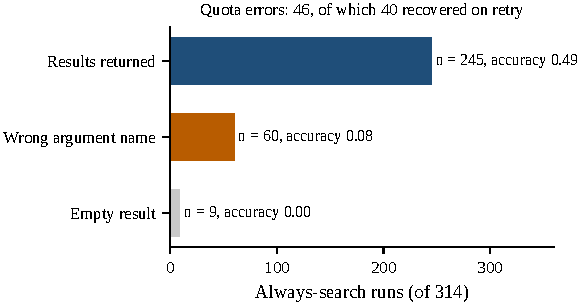
\includegraphics[width=\columnwidth]{../figures/fig4_outcomes.pdf}
\caption{Outcome of the 314 forced-search runs, classified from the recorded tool result, with judge accuracy (repeat 0) per group.}
\label{fig:outcomes}
\end{figure}

Figure~\ref{fig:outcomes} classifies each forced-search run from the recorded tool result. In 60 runs (19\%) the model called \texttt{web\_search} with the argument \texttt{search\_query}; in the base loop the harness passes the model's argument dictionary through unchanged, the search function raises a \texttt{TypeError}, and the prompt receives an error string (accuracy 0.08). Nine runs received an empty result (accuracy 0.00). Forty-six searches initially hit the SerpAPI free quota; 40 of them returned results when re-run about two hours later. An earlier version of this project reported ``114 quota failures, 112 fixed'' from a substring filter; reading the tool results corrected this. Accuracy is not explained by time sensitivity (0.41 for ``current/latest'' questions, 0.37 for fixed-year questions, 0.41 for stable ones). Across all runs, the gold answer appears in the snippets for 47\% of questions, with accuracy 0.74 when it does and 0.09 when it does not. Overall accuracy on the clean set is 0.12 without the tool and 0.50 with it (paper: 0.17 and 0.65).

\section{Limitations}
\begin{itemize}
\item One model, one task, one search engine and one prompt template; $n = 229$ questions on the clean set.
\item The judge is Qwen2.5-7B (4-bit) rather than GPT-4o; correctness was checked against a second LLM on 50 answers, not against humans. Judge outputs that failed to parse were scored as wrong and were not logged, so their number is unknown.
\item The base loop differs from the paper's chat-template harness and causes the argument-name failures; whether the results hold under the chat template is untested.
\item The clean-set rule is post hoc; we report the full set alongside. Searches ran live in October 2026 and cannot be reproduced exactly.
\item We did not run a mismatched-evidence control (another question's snippets in the same format), which would separate evidence content from position and format more directly.
\end{itemize}

\section{Conclusion and next steps}
Utility labels in this setting are consistent, so label noise does not explain why utility is hard to predict before a tool call. Reading the post-search state raises utility AUROC by about 0.15, robustly, but the gain decomposes into need (visible before the call) and answer correctness (visible after it). For tool-calling decisions this suggests a two-stage view: decide on need before the call, and use a correctness signal after the call to decide whether to trust or discard the tool output. Natural next steps are the chat-template harness, a second model and engine, a mismatched-evidence control, and human labels.

\paragraph{Reproducibility.}\raggedright Code, the regenerated result files and a dated provenance log are at \url{https://github.com/anchalrajput25/tool-utility-reliability}. \texttt{src/make\_results.py} rebuilds every reported number from the raw run files and checks it against the reported value (74 of 74 match); \texttt{src/remediation.py} runs all controls in Sec.~3.3. Raw runs are not public because they contain API request URLs.

\small
\begin{thebibliography}{9}
\bibitem[Wu et~al.(2026)]{wu2026tocall}
Qinyuan Wu, Seungeon Lee, Soumi Das, Mahsa Amani, Arijit Nag, Krishna Gummadi, Abhilasha Ravichander, and Muhammad Bilal Zafar.
\newblock To call or not to call: A framework to assess and optimize {LLM} tool calling.
\newblock \emph{arXiv:2605.00737}, 2026.

\bibitem[Kadavath et~al.(2022)]{kadavath2022know}
Saurav Kadavath et~al.
\newblock Language models (mostly) know what they know.
\newblock \emph{arXiv:2207.05221}, 2022.

\bibitem[Orgad et~al.(2025)]{orgad2025know}
Hadas Orgad, Michael Toker, Zorik Gekhman, Roi Reichart, Idan Szpektor, Hadas Kotek, and Yonatan Belinkov.
\newblock {LLMs} know more than they show: On the intrinsic representation of {LLM} hallucinations.
\newblock In \emph{ICLR}, 2025.
\end{thebibliography}
\end{document}
